\PassOptionsToPackage{hyphens}{url}
\documentclass[10pt,bibliography=totoc,listof=totoc,BCOR=5mm,DIV=10]{scrbook}
\setlength{\footheight}{36.0pt}


% use this declaration to set specific page margins
%\usepackage[a4paper , lmargin = {2.7cm} , rmargin = {2.9cm} , tmargin = {2.7cm} , bmargin = {4.6cm} ]{geometry}
\usepackage[a4paper]{geometry}
\usepackage{acronym}
\usepackage{pdflscape} % queerkant
%\usepackage{plantuml} % class diagram
%\usepackage{tikz}
%\usepackage{aeguill}
%\usepackage{svg}
\usepackage{svg}
\usepackage{amsmath}
\usepackage{csquotes} 
\usepackage{biblatex}
\addbibresource{bib/manual.bib}
\usepackage[ngerman, english]{babel}
\usepackage[ngerman]{datetime}
\usepackage{bibgerm}       		% german references
\usepackage[T1]{fontenc} % german characters
\usepackage{graphicx} 				% it's recommended to use PDF images but you can use JPG or PNG as well
\usepackage[hyphens]{url}
%\usepackage{hyperref}
%\usepackage{url}           		% format URLs
%\usepackage{hyperref} 				% create hyperlinks
\usepackage{listings, color}	% for source code
\usepackage{subfig}						% two figures next to each other (example: figure 3a), figure 3b)
\usepackage{scrlayer-scrpage}					% header and footer line
\usepackage{todonotes}
% header and footer line - no header & footer line on pages where a new chapter starts
%\usepackage{float} % Float H
\usepackage{amssymb} % Math G
\usepackage{amsmath} %Equations
\usepackage[hypcap=false]{caption} % for fixing a warning
\usepackage{algorithm}
\usepackage{algpseudocode}
\usepackage{url}
\usepackage[strings]{underscore}
\usepackage{hyperref}
\usepackage{xurl}
\usepackage{cleveref}
\usepackage{enumitem}
\usepackage{dirtytalk}
\pagestyle{scrheadings}
\ohead{\headmark}%Design and Implementation of X}
\ihead{Ramon Mehrpoya}
\ofoot[]{\thepage}
\setlength{\footheight}{27.2pt} 
\ifoot{Verifiable Decentralized Federated Machine \\ Learning and Inference for AI Agent Systems\\TU Berlin, Software and Business Engineering, 2026}

% set path where images are stored
\graphicspath{{./img/}}

%\input{./misc/hyphenation} 					% use this file to set explicit hyphenations (doesn't seem to work correctly)
\usepackage{colortbl} % Tabellenfarben


\newdateformat{myformat}{\THEDAY. \monthnamengerman[\THEMONTH] \THEYEAR}

\definecolor{codegreen}{rgb}{0,0.6,0}
\definecolor{codegray}{rgb}{0.5,0.5,0.5}
\definecolor{codepurple}{rgb}{0.58,0,0.82}
\definecolor{backcolour}{rgb}{0.95,0.95,0.92}

%\lstdefinestyle{mystyle1}{
%    backgroundcolor=\color{backcolour},   
%    commentstyle=\color{codegreen},
%    keywordstyle=\color{magenta},
%    %numberstyle=\tiny\color{codegray},
%    stringstyle=\color{codepurple},
%    basicstyle=\ttfamily\tiny,
%    breakatwhitespace=false,         
%    breaklines=true,                 
%    captionpos=b,                    
%    keepspaces=true,                 
%    %numbers=left,                    
%    %numbersep=5pt,                  
%    showspaces=false,                
%    showstringspaces=false,
%    showtabs=false,                  
%    tabsize=2,
%    moredelim=**[is][\color{red}]{*|}{|*}
%}

%\lstdefinestyle{mystyle2}{
%    backgroundcolor=\color{backcolour},   
%    commentstyle=\color{codegreen},
%    keywordstyle=\color{magenta},
%    numberstyle=\tiny\color{codegray},
%    stringstyle=\color{codepurple},
%    basicstyle=\ttfamily\tiny,
%    breakatwhitespace=false,         
%    breaklines=true,                 
%    captionpos=b,                    
%    keepspaces=true,                 
%    numbers=left,                    
%    numbersep=5pt,                  
%    showspaces=false,                
%    showstringspaces=false,
%    showtabs=false,                  
%    tabsize=2,
%    moredelim=**[is][\color{red}]{*|}{|*}
%}

%\DeclareCiteCommand{\bracketcite}[\mkbibbrackets]
%  {\usebibmacro{prenote}}
%  {\usebibmacro{citeindex}%
%   \usebibmacro{cite}}
%  {\multicitedelim}
%  {\usebibmacro{postnote}} 

\begin{document}
% ---------------------------------------------------------------
\frontmatter
    \thispagestyle{empty}
\begin{center}

%\vspace*{1cm}
{\LARGE \textbf{Technische Universität Berlin}}


\vspace*{1cm}


\includegraphics[width=4cm]{images/tu_logo.eps}
% \begin{figure}
%     \centering
%     
\includegraphics[width=1\linewidth]{images/tu_logo.eps}
%     \caption{Enter Caption}
%     \label{fig:placeholder}
% \end{figure}
\vspace*{1.0cm}

{\LARGE Master's Thesis}\\

\vspace{0.5cm}
{\huge \textbf{Verifiable Decentralized Federated \\ Machine Learning and Inference \\ for AI Agent Systems}}\\

\vspace{2.1cm}



Written by:\\
Ramon Mehrpoya\\
Matriculation Number: 371968\\
%ramon.mehrpoya@campus.tu-berlin.de\\
Technische Universität Berlin, Germany\\
\today\\ 
\vspace{1cm}
 
Supervised by:\\
%Prof. Dr.-Ing. Stefan Tai\\
%Prof. Dr.-Ing. Stefan Schulte\\
Dr.-Ing. Jonathan Johannes Heiß\\
Software and Business Engineering\\
Technische Universität Berlin, Germany
\vspace{0.8cm}

Examiner 1:\\
Prof. Dr.-Ing. Stefan Schulte\\
Software and Business Engineering\\
Technische Universität Berlin, Germany
\vspace{0.8cm}

Examiner 2:\\
Prof. Dr.-Ing. Stefan Tai\\
Information Systems Engineering\\
Technische Universität Berlin, Germany
\vspace{0.8cm}
\end{center}




    %\thispagestyle{empty}
    %\cleardoublepage
    
    
    %\include{./misc/self-assertion} 
    %\thispagestyle{empty}
    %\cleardoublepage

    %\newpage

\thispagestyle{empty}

\begin{large}

\vspace*{6cm}

\noindent
Hiermit erkläre ich, dass ich die vorliegende Arbeit selbstständig und eingenhändig sowie ohne unerlaubte fremde Hilfe und ausschließlich unter Verwendung der aufgeführten Quellen und Hilfsmittel angefertigt habe.

\vspace{2cm}

\noindent
Berlin, den \myformat\today

\vspace{3cm}

\hspace*{7cm}%
\dotfill\\
\hspace*{8.5cm}%
\textit{(Unterschrift)}

\end{large}
 
    %\thispagestyle{empty}
    %\cleardoublepage
    
    
    %\thispagestyle{empty}
\vspace*{1.0cm}

\begin{center}
    \textbf{Abstract}
\end{center}

\vspace*{0.5cm}

\noindent

This thesis shows how to extend ZoKrates by further embedded elliptic curves. It gives an introduction to elliptic curve arithmetic, to familiarize the reader with the terminology. It introduces SageMath code for finding an embedded curve and evaluating possible candidates using the SafeCurve criteria. A detailed implementation of the BLS12\_377s embedded curve, the Decaf377, is presented, as well as an EdDSA signature verification using the newly implemented Decaf377 nested inside the BLS12\_377 in turn nested in a BW6\_761. Then results of the SafeCurve criteria test on implemented and possible curves for ZoKrates is presented and I explain why the possible implementation of the Bandersnatch, an embedded curve of the BLS12\_381, is ruled out. I will give an overview of embedded elliptic curves, in the context of zk-SNARKs, with ZoKrates and thereby will facilitate the implementation of new embedded elliptic curves for non-crypto experts.

    %\thispagestyle{empty}
    %\cleardoublepage
    
    %\thispagestyle{empty}
\vspace*{0.2cm}

\begin{center}
    \textbf{Zusammenfassung}
\end{center}

\vspace*{0.2cm}

\noindent 
Diese Arbeit zeigt, wie ZoKrates um weitere eingebettete elliptische Kurven erweitert werden kann. Sie gibt eine Einführung in die Arithmetik  von elliptischen Kurven, um sich mit der erforderlichen Terminologie vertraut zu machen.
Dann wird ein SageMath code vorgestellt um eingebettete Kurven zu finden und um mögliche Kandidaten anhand der SafeCurve-Kriterien zu bewerten. Es wird eine detaillierte Implementierung einer eingebetteten Kurve der BLS12\_377s namens Decaf377, sowie eine Signaturüberprüfung in Form einer EdDSA Signatur in der Decaf377 vorgestellt, die innerhalb der BLS12\_377 verschachtelt und wiederum in eine BW6\_761 verschachtelt ist. Anschließend präsentiere ich meine Ergebnisse der SafeCurve Kriterien von bereits implementierten und möglichen zukünftigen Kurven für ZoKrates und schließe die mögliche Implementierung der Bandersnatch, einer eingebetteten Kurve der BLS12\_381, aus. Ich werde einen Überblick über eingebettete elliptische Kurven im Kontext von zk-SNARKs geben und damit die Implementierung neuer eingebetteten elliptischen Kurven für Nicht-Krypto-Experten erleichtern.
    %\thispagestyle{empty}
    
    
    \tableofcontents
    %\thispagestyle{empty}
    
    %\listoffigures
    %\thispagestyle{empty}
    
    %\listoftables
    %\thispagestyle{empty}
    
% --------------------------------------------------------------

\mainmatter % comment single chapters for faster compilation

    \chapter{Introduction}
\label{cha:chapter1}

\section{Introduction}

Recent advances in \ac{AI} have led to the emergence of agent-based systems in which autonomous \ac{AI} agents act as interfaces between users and complex computational services. These agents are capable of decomposing tasks, interacting with external tools, and integrating multiple data sources and models to support decision-making. In critical application domains such as healthcare, such systems hold significant potential. For instance, medical professionals may rely on \ac{AI} agents to analyze medical data such as X-ray or MRI images and assist in diagnosis.

\subsection{Motivation}

To illustrate this scenario, consider a physician interacting with an \ac{AI} agent to analyze medical images. Instead of relying on a general-purpose model, the agent dynamically retrieves a specialized model via standardized interfaces. This model may have been trained across multiple hospitals, leveraging a diverse set of sensitive medical datasets without exposing raw data. During inference, the agent can provide additional guarantees by leveraging verifiable \ac{ML} techniques to ensure that predictions were produced with respect to the intended model. At the same time, attestation mechanisms can be used to verify that relevant parts of the training process were executed under trusted conditions and, if necessary, with the intended code.

This combination enables not only accurate predictions, but also verifiable guarantees regarding the origin, integrity, and correctness of both the model training and its outputs.

From a system perspective, the integration of decentralized machine learning into real-world applications requires considering multiple abstraction layers. At the application layer, users interact with \ac{AI} agents that provide task-specific functionality, such as medical decision support. At the service and orchestration layer, these agents coordinate access to external models, data sources, and computational services. Beneath this, the model layer is responsible for providing trained machine learning models, including mechanisms for model retrieval, execution, and lifecycle management. At the infrastructure layer, \ac{DFL}, blockchain systems, and \acp{TEE} enable distributed training, coordination, and trusted execution.

While existing work often focuses on individual layers in isolation, ensuring trustworthiness across the entire system requires a holistic view that spans all layers. In particular, guarantees established at the infrastructure level, such as secure execution through \acp{TEE}, must be propagated to the application layer, where decisions are made based on model predictions. This highlights the need for end-to-end approaches that connect decentralized training, verifiable computation, and agent-based interaction within a unified system architecture.


\subsection{Problem Statement}

However, such scenarios introduce a fundamental challenge. While \ac{AI} agents provide flexible and powerful interaction mechanisms, they often depend on components whose origin, integrity, and correctness cannot be readily verified. In safety-critical environments, it is not sufficient to obtain a prediction; the underlying model, its provisioning process, and the correctness of its execution must also be trustworthy. In particular, it is necessary to establish verifiable guarantees regarding model provenance, the integrity of training and aggregation steps, and the correctness and reproducibility of inference results with respect to the intended model.

\ac{FL} was introduced as a promising paradigm for collaborative \ac{ML} in distributed environments, where multiple participants jointly train a global model without sharing their raw data \cite{mcmahan2017communication}. This enables institutions such as hospitals to train models on sensitive data while preserving privacy collaboratively. However, traditional \ac{FL} systems rely on centralized coordination and therefore introduce trust assumptions regarding the central aggregator.

To overcome these limitations, \ac{DFL} distributes the training process across multiple participants. While this removes single points of failure, it introduces new challenges related to coordination, robustness, and trust. In particular, in the absence of a trusted central entity, it becomes difficult to ensure that training is executed correctly and that participating nodes behave honestly.

\subsection{Limitations of Existing Approaches}

To address these issues, prior work has explored the integration of \ac{DFL} with \acp{TEE} and verifiable computation. For example, \cite{heiss2022verifiable, 10634412} propose a framework for blockchain-based federated learning with verifiable off-chain computation. Building upon this approach, \cite{hartmann2024dfl} presents a prototype implementation that combines \ac{DFL}, \ac{TEE}-based attestation, and zero-knowledge proofs.

While this prototype demonstrates the feasibility of verifiable training, it abstracts away several aspects required for practical deployment. In particular, attestation verification is simplified and partially simulated, and system-level concerns such as robustness and complete coordination logic are not fully addressed.

At the same time, recent advances in verifiable \ac{ML} have introduced approaches for attesting the correctness of model inference. These techniques allow the generation of cryptographic proofs that a prediction was computed correctly with respect to a fixed model. However, such approaches are typically limited to non-distributed systems \cite{10.1145/3627703.3650088, south2024verifiableevaluationsmachinelearning}.


Furthermore, recent developments in \ac{AI} highlight a growing trend toward agentic systems that interact with external tools and models (e.g., systems such as OpenClaw\footnote{\url{https://github.com/openclaw/openclaw}}, frameworks such as LangChain\footnote{\url{https://github.com/langchain-ai/langchain}}, Microsoft AutoGen\footnote{\url{https://github.com/microsoft/autogen}}, CrewAI\footnote{\url{https://github.com/crewAIInc/crewAI}}, LlamaIndex\footnote{\url{https://github.com/run-llama/llama_index}}, or OpenHands\footnote{\url{https://github.com/All-Hands-AI/OpenHands}}). While these systems enable flexible interaction with \ac{ML} models, they typically lack guarantees regarding the origin, integrity, and correctness of the utilized models.

\subsection{Research Gap}

In particular, the end-to-end trust chain, from training and model publication to model retrieval and inference, remains incomplete for \ac{DFL} models. Existing work either focuses on \ac{DFL} training or on centralized \ac{ML} training with inference assurances, but does not provide an approach focusing on \ac{DFL} training with inference assurances. The main reason for this being: \say{In the context of distributed machine learning, decentralized algorithms have long been treated as a compromise — when the underlying network topology does not allow centralized communication, one has to resort to decentralized communication, while, understandably, paying for the cost of being decentralized.}, according to \cite{lian2017can}.

This gap becomes particularly critical when combining agent-based systems with \ac{DFL}. While \ac{DFL} enables the training of specialized models on decentralized and sensitive data, there is currently no established approach that integrates such models into agent-based systems in a verifiable manner for \ac{DFL} trained models.

\subsection{Research Questions}

This thesis addresses this challenge by investigating how \ac{DFL} models can be integrated into \ac{PAA}/agent-based system architectures while ensuring trustworthiness across the entire pipeline. The goal is to enable agents to not only utilize trained models for task-specific inference, but also to provide verifiable guarantees about the provenance, integrity, and correctness of these models and their outputs.

In particular, the following \acp{RQ} are considered:

\begin{description}
    \item[\textbf{\ac{RQ} 1:}] How can \ac{DFL} models be integrated into \ac{AI} agent-based system architectures while ensuring trustworthiness across the entire training and inference pipeline?

    \begin{description}
        \item[\textbf{\ac{RQ} 1.1:}] How can verifiable \ac{DFL} guarantee integrity and availability during model training?
        
        \item[\textbf{\ac{RQ} 1.2:}] How can \ac{ML} inference be made verifiable, such that the integrity of model predictions can be guaranteed, for example through cryptographic proofs of execution?
    \end{description}
\end{description}

\subsection{Research Approach}

To address the proposed \acp{RQ}, this thesis follows a system-oriented and artifact-based research approach. The work combines architecture design, prototype implementation, and experimental evaluation. The central research artifact is a reproducible prototype that connects decentralized model training, smart-contract-based coordination, model provenance, artifact retrieval, and verifiable inference within an agent-oriented system setting.

The research is conducted in three steps. First, a layered architecture is designed that identifies the relevant system components and trust relationships between decentralized training, blockchain-based metadata management, artifact storage, agent-based model retrieval, and verifiable inference. Second, the architecture is implemented as a proof-of-concept prototype using Docker Compose, smart contracts, local \ac{IPFS} storage, \ac{DFL} workers, an agent orchestration layer, and a zero-knowledge inference pipeline. Third, the prototype is evaluated with respect to functionality, feasibility, reproducibility, runtime overhead, and the extent to which selected trust properties can be established across the pipeline.

To address \textbf{\ac{RQ} 1}, the thesis investigates how a \ac{DFL}-trained model can be made available to an \ac{AI} agent in a trustworthy manner. The prototype connects decentralized training and aggregation with on-chain model metadata, content-addressed artifact storage, and an agent that retrieves the current model based on smart-contract state. The evaluation focuses on whether the agent can identify the intended model, retrieve the corresponding artifacts, verify their integrity, and initiate verifiable inference without relying solely on off-chain assumptions.

To address \textbf{\ac{RQ} 1.1}, the thesis investigates how selected integrity and availability properties of \ac{DFL} training can be supported. The implementation extends a \ac{DFL} prototype with smart-contract-based device registration, aggregator coordination, model metadata storage, \ac{TEE}-related attestation flows, \ac{IPFS}-based artifact publication, and cryptographic binding between model artifacts and the responsible aggregator. The evaluation analyzes the correctness and scope of these mechanisms, including successful training and aggregation runs, model publication, signature verification, aggregator registration, failure handling, and the overhead introduced by on-chain coordination and verification.

To address \textbf{\ac{RQ} 1.2}, the thesis investigates how inference over a retrieved \ac{DFL} model can be made verifiable in an agent-based setting. The prototype integrates an agent component that reads model metadata from the blockchain, fetches model and signature artifacts from \ac{IPFS}, verifies the artifact signature against the registered aggregator, and invokes a zero-knowledge inference service. The evaluation analyzes whether a proof can be generated and verified for a single-image inference query, how this proof relates to the referenced model artifact, and what computational overhead is introduced by the proof generation and verification pipeline.

The evaluation uses a healthcare-inspired scenario as motivation but relies on MNIST image classification as a reproducible proof-of-concept workload. This choice allows the thesis to focus on system integration and verifiability rather than medical model performance. Accordingly, the evaluation does not claim clinical validity, production readiness, or complete protection against all adversarial behavior. Instead, it assesses which trust properties can be demonstrated by the implemented architecture and where remaining assumptions and limitations persist.



\section{Background}

To address the challenges outlined in the previous section, this thesis builds upon several key technologies. The following subsections introduce these foundational concepts and highlight their role within the proposed system.

\subsection{Federated and Decentralized Learning}

\ac{FL} enables collaborative model training without sharing raw data, typically using aggregation algorithms such as Federated Averaging \cite{mcmahan2017communication}. This allows multiple participants to jointly train a global model while preserving data privacy.

To overcome the limitations of centralized coordination, \ac{DFL} distributes the training process among participating nodes. While this improves robustness and removes single points of failure, it introduces new challenges such as the absence of a trusted coordinator, difficulties in verifying participants, and an increased risk of malicious behavior \cite{Kalapaaking_2023}.

\subsection{Trusted Execution Environments and Attestation}

To establish trust in decentralized environments, \acp{TEE} provide a hardware-based mechanism for secure execution. \acp{TEE} are defined as secure areas of a processor that guarantee the confidentiality and integrity of code and data loaded within them \cite{sabt2015trusted}.

Remote attestation enables external parties to verify that a specific piece of code was executed within a valid \ac{TEE}. In this work, Intel \ac{DCAP}-based attestation is considered as a basis for providing such guarantees, in particular through quote-based verification of measured execution environments \cite{10.1145/3652597}. This forms an important basis for increasing trust in the execution environment and software identity of training processes in \ac{DFL} systems, although it does not by itself prove the authenticity of input data or the full semantic correctness of training outcomes.

A central artifact in such an attestation flow is the quote. In the case of Intel TDX-style attestation, a quote contains a header, a measured report body, and signature-related certification data.\footnote{\url{https://download.01.org/intel-sgx/latest/dcap-latest/linux/docs/Intel_TDX_DCAP_Quoting_Library_API.pdf}} The header identifies properties such as the quote version, attestation key type, TEE type, and quote enclave vendor. The report body contains security-version information and measurements of the trusted domain, including values such as the \ac{TEE} \ac{TCB} \ac{SVN}, \ac{MRTD}, \ac{MRSEAM}, \ac{MRCONFIGID}, \ac{MROWNER}, \ac{MROWNERCONFIG}, runtime measurement registers such as \ac{RTMR}0--\ac{RTMR}3, and application-controlled report data.\footnote{\url{https://docs.phala.com/phala-cloud/attestation/attestation-fields}} These values are not meaningful in isolation; they become useful because they are included in data that is cryptographically signed and can therefore be checked by a verifier.

In practical \ac{TEE} quote verification, the attestation result is not established by a single cryptographic check, but by a chain of signature, hash, certificate, and collateral validations. For an Intel TDX/\ac{DCAP}-style quote, a verifier typically checks the quote signature over the signed quote data, verifies that the attestation key is bound to the \ac{QE} report through a hash over the attestation key and \ac{QE} authentication data, verifies the \ac{QE} report signature, and validates the \ac{PCK} certificate chain.\footnote{\url{https://download.01.org/intel-sgx/latest/dcap-latest/linux/docs/Intel_TDX_DCAP_Quoting_Library_API.pdf}} In an implementation using a three-certificate \ac{PCK} chain, this can amount to approximately two direct P-256/ECDSA signature checks for the quote and \ac{QE} report, up to three additional certificate-chain signature checks, and several SHA-256 computations for signed message digests, certificate bodies, and key-binding checks. Further checks are not signature verifications, but are still security-critical: certificate validity periods, revocation information, Intel collateral lookup, \ac{QE} identity validation, and \ac{TCB}-level evaluation. The exact number of operations may vary depending on the certificate chain, available collateral, revocation data, and whether parts of the verification result are cached. These checks establish authenticity of the quote and acceptability of the platform state, but they do not by themselves prove that a particular application, Docker image, or source commit was executed.

At a minimum, quote verification checks whether the quote is structurally valid, whether it belongs to the expected \ac{TEE} and quote version, whether the quote body is signed by a valid attestation key, and whether this attestation key is bound to Intel-backed certification data. In a \ac{DCAP}-based verification flow, this includes verifying the quote signature over the quote header and report body, verifying the report of the quote enclave, checking the \ac{PCK} certificate chain against Intel collateral, and evaluating the platform's \ac{TCB} status.\footnote{\url{https://www.intel.com/content/www/us/en/developer/tools/trust-domain-extensions/documentation.html}} Such a minimal verification can establish that a quote was produced by a valid attestation flow on a platform with an acceptable \ac{TCB} state and that the measured report body was not modified after signing.

However, these checks do not automatically imply that a semantically intended workload was executed. Measurements such as \ac{MRTD} or \ac{RTMR} values are hashes or hash-chain results, not human-readable descriptions of source code. A verifier must compare them against expected reference values to derive stronger claims. For example, a verifier may require a specific \ac{MRTD} value or a set of approved runtime measurements. Without such a measurement policy, attestation can show that the quote is authentic and bound to a measured TEE state, but not necessarily that this state corresponds to a particular application selected by the verifier.

The same distinction applies to containerized deployments. A TEE quote can support evidence that a specific Docker-based application configuration was launched if the deployment platform measures the configuration into runtime measurement registers. In Phala/dstack-style deployments, for instance, \ac{RTMR}3 can be used as an application-specific measurement chain that includes deployment metadata such as an application identifier and a compose hash.\footnote{\url{https://docs.phala.com/phala-cloud/attestation/verify-your-application}} To verify a concrete YAML file, a verifier would need the expected Docker Compose configuration, recompute the corresponding compose hash, replay or validate the runtime measurement log, and compare the resulting \ac{RTMR}3 value with the value contained in the quote.

Verifying a specific Docker image requires an additional condition: the YAML file should reference immutable image digests instead of mutable tags. An image reference such as \texttt{app:latest} is insufficient because the tag may later point to different image contents. In contrast, a reference such as \texttt{app@sha256:<digest>} binds the configuration to a concrete image digest.\footnote{\url{https://docs.docker.com/dhi/core-concepts/digests/}} To further connect this image to source code, the image digest must be linked to a trusted build process, for example through reproducible builds, signed container images, software bills of materials, or build provenance generated by a continuous integration pipeline \cite{236322}. The resulting trust chain can be summarized as follows:

\begin{center}
\texttt{source commit -> trusted build -> image digest -> compose file -> compose hash -> \ac{RTMR}3 -> TEE quote}
\end{center}

Consequently, this thesis treats TEE attestation as a mechanism for establishing selected execution-environment and measurement guarantees, not as a complete proof of application correctness. A minimal attestation design can verify quote authenticity, certificate validity, and \ac{TCB} acceptability. Stronger guarantees, such as proving that a specific YAML file, Docker image, or source commit was used, require additional measurement policies, immutable image references, and build provenance. These stronger checks are therefore considered part of the design space and evaluation scope, rather than assumed to be automatically provided by the quote itself.



\subsection{Verifiable Computation and Zero-Knowledge Proofs}

One approach to making computation verifiable in decentralized systems is the use of \acp{ZKP}. Systems such as the RISC Zero \ac{zkVM} allow programs to be executed off-chain while generating cryptographic proofs of correct execution.

These proofs can be transformed into Groth16 zk-SNARKs, which are efficiently verifiable on-chain. This typically involves a STARK-to-SNARK transformation, where zk-STARK-based execution traces are compressed into proofs suitable for verification in the \ac{EVM}\footnote{\url{https://dev.risczero.com/api/blockchain-integration/risc-zero-on-eth}}.

While this approach provides strong verifiability guarantees, it introduces significant computational overhead and system complexity, making it challenging to apply in practical large-scale systems.

\subsection{Blockchain-Based Coordination and Storage}

As an alternative or complement to full verifiable computation, this thesis considers direct cryptographic verification on-chain. Smart contracts, originally conceptualized by Nick Szabo as self-executing agreements \cite{szabo1997smart}, became practically feasible with the introduction of Bitcoin \cite{nakamoto2008bitcoin}.

Modern platforms such as Ethereum extend this concept by enabling programmable smart contracts within the \ac{EVM}, allowing decentralized coordination without a central authority. In addition, \ac{IPFS} provides decentralized storage through content addressing, which is particularly suitable for storing model updates and global models in \ac{DFL} systems.

Efficient on-chain verification of cryptographic primitives is a key challenge. The introduction of \ac{RIP}-7212\footnote{\url{https://ethereum-magicians.org/t/eip-7212-precompiled-for-secp256r1-curve-support/14789}} and later \ac{EIP}-7951\footnote{\url{https://eips.ethereum.org/EIPS/eip-7951}} enables native precompile support for the secp256r1 elliptic curve on networks such as Mainnet, Sepolia, Hoodi, and Holesky since the Fusaka/Osaka upgrade at the end of 2025\footnote{\url{https://stakely.io/blog/all-about-ethereum-fusaka-upgrade-and-its-12-eips}}. 

Unlike Ethereum's default secp256k1 curve, secp256r1 is widely used in hardware-based security systems such as WebAuthn and secure enclaves\footnote{\url{https://www.w3.org/TR/webauthn-2/}}. Native support via precompiled contracts significantly reduces the cost of signature verification, which is particularly relevant for on-chain \ac{TEE} attestation.


\subsection{Specialized Neural Network Models vs Large Language Models}

\acp{NN} in general are based on computational models inspired by the structure of biological neurons, see Figure \ref{fig:nn}. 

\begin{figure}[ht!]
    \centering
    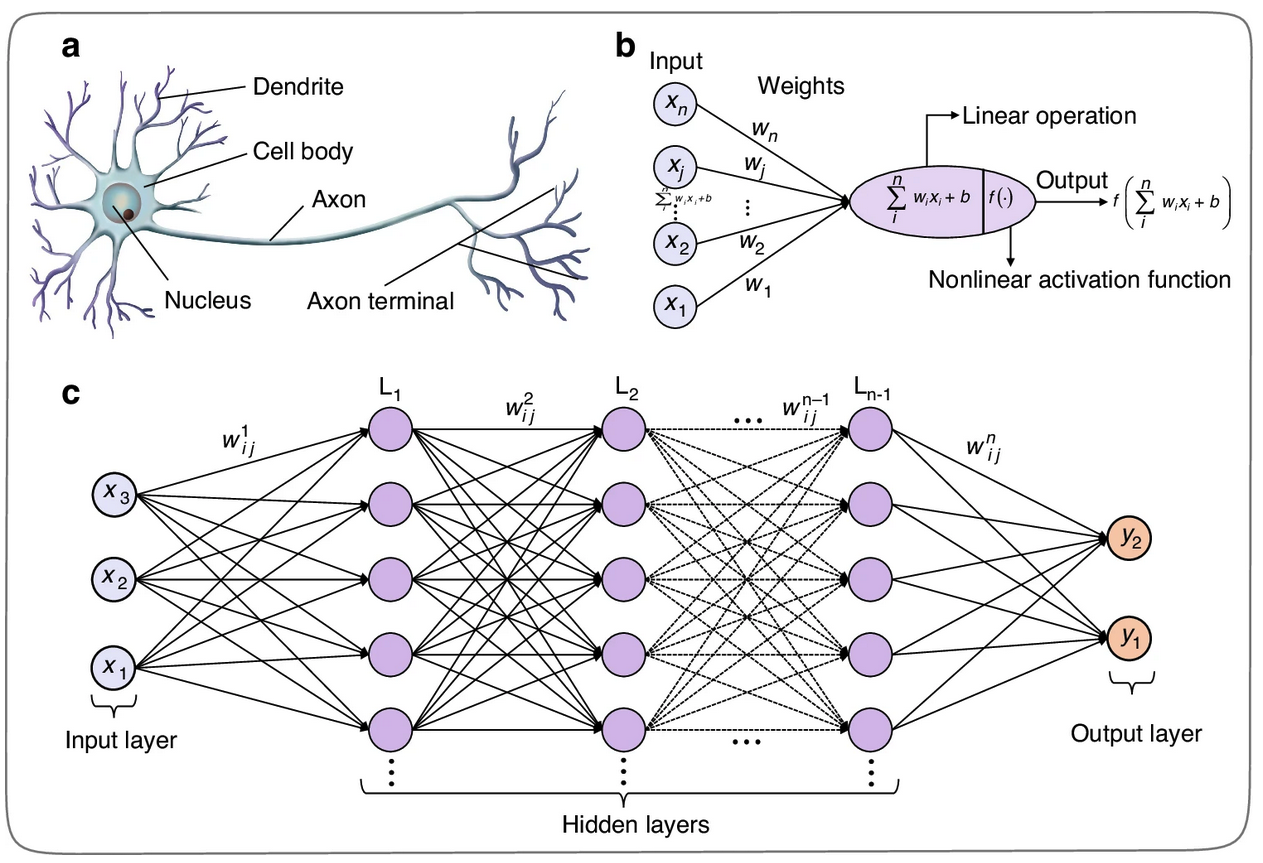
\includegraphics[width=1\linewidth]{images/Bildschirmfoto 2026-05-07 um 11.05.57.png}
    \caption{Neuron structure and artificial neural network. a Structure of biological neurons. b Mathematical inferring process of artificial neurons in multi-layer perceptron, including the input, weights, summation, activation function, and output. c Multi-layer perceptron artificial neural network\protect\footnotemark[8]}
    \label{fig:nn}
\end{figure}
\footnotetext[8]{\url{https://www.nature.com/articles/s41377-024-01590-3/figures/3}}
\setcounter{footnote}{8}



They learn complex patterns from data by adjusting internal parameters during training and are widely used for tasks such as image classification, speech recognition, and natural language processing.

Different \ac{NN} architectures are optimized for different tasks. \acp{CNN} \cite{fukushima1980neocognitron}, for example, are commonly used for image analysis, see Figure \ref{fig:cnn}, while Transformer-based architectures \cite{vaswani2023attentionneed} have become the dominant approach for language processing.

\acp{LLM} are large-scale \acp{NN} trained on massive text corpora to perform general-purpose language understanding and generation tasks. Due to their broad training data and reasoning capabilities, \acp{LLM} form the foundation of many modern agent-based systems.

However, despite their flexibility, general-purpose \acp{LLM} are not always optimal for specialized domain-specific tasks. In areas such as healthcare, dedicated \acp{CNN} architectures remain widely used for applications such as medical image classification and signal analysis due to their task-specific design and computational efficiency \cite{CHEN2025109507}.

\begin{figure}[ht!]
    \centering
    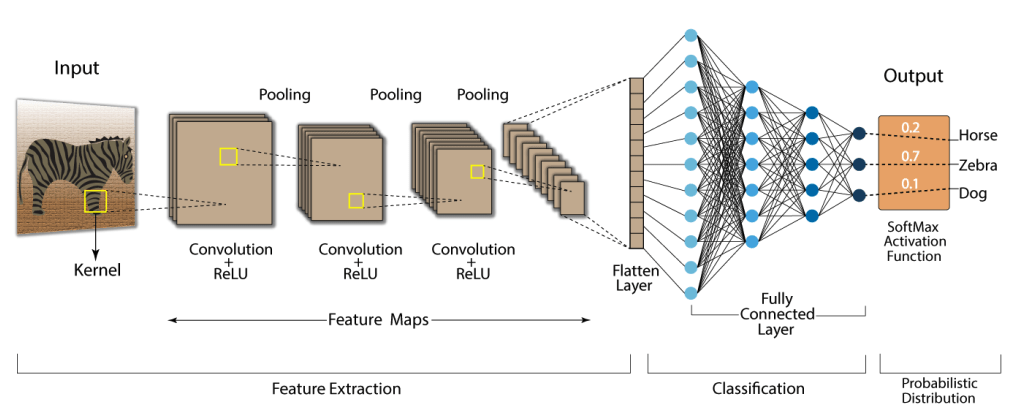
\includegraphics[width=1\linewidth]{images/Bildschirmfoto 2026-05-10 um 00.18.40.png}
    \caption{Convolutional Neural Network \protect\footnotemark[9]}
    \label{fig:cnn}
\end{figure}
\footnotetext[9]{\texttt{\url{https://i0.wp.com/developersbreach.com/wp-content/uploads/2020/08/cnn\_banner.png?fit=1024\%2C481\&ssl=1}}}
\setcounter{footnote}{9}

\ac{DFL} enables such specialized models to be trained collaboratively across multiple institutions without requiring centralized data collection. In \ac{DFL} environments, these models can therefore capture distributed domain-specific knowledge while preserving privacy \cite{10634412}.


In the context of this thesis, \acp{LLM} are primarily used as orchestration and interaction components within agent systems, while specialized \ac{NN} models trained through \ac{DFL} are used for task-specific inference. Depending on the evaluation scenario, the implemented models may include both fully \acp{NN} or \acp{CNN}, especially for image classification tasks.

\subsection{AI Agents, MCP and RAG}

Beyond secure training and verification, the coordination and utilization of decentralized systems can be enhanced through autonomous software entities. 
A \ac{PAA} can be defined as an \ac{AI} system that utilizes \acp{LLM} as its central decision-making component to decompose complex user requests into executable subtasks and solve them autonomously using external tool\textsuperscript{9}, as illustrated in Figure~\ref{fig:agent-overview}.

Recent developments emphasize the integration of specialized models and external data sources into agent workflows. In contrast to general-purpose \acp{LLM}, these models can be trained on domain-specific data, for example via \ac{DFL}.

To enable interaction with such external components, modern agent systems rely on standardized interfaces such as the \ac{MCP}, which allows agents to dynamically load and interact with external tools, models, and services. Additionally, \ac{RAG} enables agents to retrieve relevant information from external data sources (e.g., databases or blockchains) and incorporate it into their reasoning process.

In this context, \ac{PAA} acts as an interface between users and decentralized learning systems. They can load trained models via \ac{MCP}, execute inference, and augment results with verifiable metadata, such as attestation records retrieved from the blockchain using \ac{RAG}. This enables not only task-specific predictions, but also validation of model origin and integrity.

\begin{figure}[ht!]
    \centering
    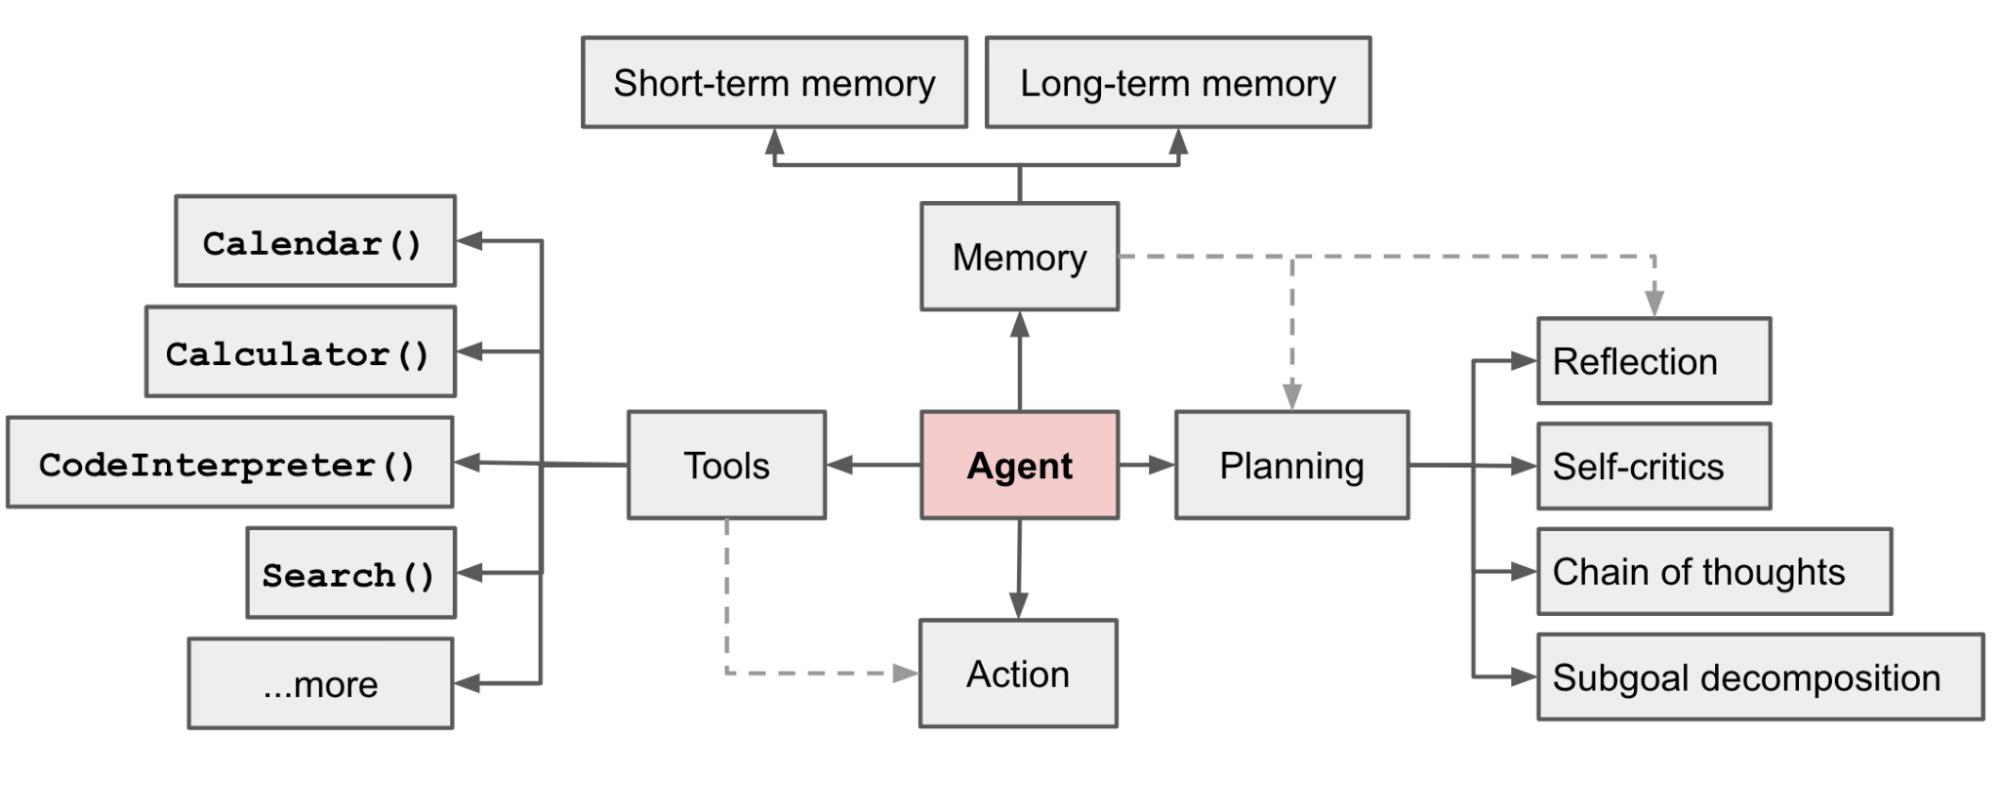
\includegraphics[width=1\linewidth]{images/agent-overview.png}
    \caption{Overview of a LLM-powered autonomous agent system\protect\footnotemark[10]}
    \label{fig:agent-overview}
\end{figure}
\footnotetext[10]{\url{https://lilianweng.github.io/posts/2023-06-23-agent/}}
\setcounter{footnote}{10}

\subsection{Machine Learning Inference and Verifiability}

\ac{ML}inference refers to the process of applying a trained model to new input data in order to generate predictions or decisions. In contrast to the training phase, inference represents the operational stage in which models are deployed and used in real-world applications.

In many scenarios, inference is the primary point of interaction between users and \ac{ML} systems. For example, in medical applications, models are used to classify X-ray images or support diagnostic decisions, making correctness and reliability critical.

However, traditional systems provide limited guarantees regarding inference integrity. In particular, users typically cannot verify whether the correct model was used, whether the model has been tampered with, or whether the prediction was computed faithfully.

These challenges are amplified in decentralized and agent-based systems, where inference may involve multiple components and external services. Ensuring trust in such environments requires mechanisms that go beyond conventional execution.

Recent research explores verifiable \ac{ML} approaches that provide cryptographic guarantees about inference correctness \cite{10.1145/3627703.3650088, south2024verifiableevaluationsmachinelearning}. Techniques such as zero-knowledge proofs and verifiable computation enable a prover to demonstrate that a prediction was computed correctly without revealing sensitive data.

While promising, these approaches are not yet fully adapted to distributed and agent-based environments. Consequently, enabling efficient and verifiable inference in such systems remains an open research challenge.

In this thesis, inference is considered as part of an end-to-end pipeline, including decentralized training, trusted model provisioning, and agent-based model usage. This perspective highlights the need for mechanisms that ensure not only correct predictions but also the integrity and provenance of the underlying models.
\newpage

\section{Related Work}

This section reviews existing research related to \ac{DFL} and its integration into modern \ac{AI} systems. The focus lies on system architectures, trust mechanisms, and the practical usability of trained models. The literature is structured into three main areas. Verifiable \ac{DFL}, including \acp{TEE}-based approaches, verifiable \ac{ML} inference, and \ac{AI} agents and tool-augmented systems. The goal is to identify limitations in current approaches and highlight gaps in the state of the art.

\subsection{Verifiable Decentralized Federated Learning}

\ac{DFL} has been widely studied as an alternative to centralized training, aiming to remove single points of failure and improve system robustness. However, recent surveys show that decentralization introduces significant challenges in coordination, trust establishment, and verification of participating nodes \cite{martinezbeltran2023decentralized}.

To address these challenges, blockchain-based approaches have been proposed to enable transparent coordination and auditability of training processes \cite{qu2023blockchainfl}. In particular, verifiable federated learning systems aim to ensure the correctness of off-chain computations. For example, \cite{heiss2022verifiable, 10634412} introduces a framework that combines \ac{DFL} with blockchain-based verification of off-chain execution.


Building upon this approach, \cite{hartmann2024dfl} presents a prototype that integrates decentralized training, smart contract-based coordination, and \ac{TEE}-based attestation within a \ac{zkVM}-based verification pipeline. The prototype utilizes a relatively simple machine learning setup based on the MNIST dataset and a fully connected feedforward \ac{NN} (\ac{MLP}). In this architecture, a flattened 28$\times$28 pixel image is represented as a vector of 784 input values and processed through multiple dense hidden layers before producing a prediction for one of the ten handwritten digit classes. Unlike \acp{CNN}, which explicitly exploit spatial image structures, the employed network treats the image as a plain vector of numerical values.

While this work demonstrates the feasibility of combining \ac{DFL}, blockchain-based coordination, and hardware-based trust mechanisms, it abstracts away several aspects required for practical deployment. In particular, attestation verification is simplified, and system-level concerns such as robustness and complete coordination logic are not fully addressed.

More importantly, existing approaches primarily focus on securing the training process itself. The question of how trained verifiable \ac{DFL} models can be used in a verifiable and trustworthy manner after deployment remains largely unaddressed.

\subsection{Verifiable Machine Learning Inference}

Recent advances in verifiable computation have led to increasing interest in verifiable \ac{ML} inference. The goal of these approaches is to provide cryptographic guarantees that a prediction was computed correctly with respect to a given model.

Several works propose the use of zero-knowledge proofs (ZKPs) to verify \ac{NN} inference. Systems such as ZKML\footnote{\url{https://github.com/ddkang/zkml}} and EZKL\footnote{\url{https://github.com/zkonduit/ezkl}} enable the generation of proofs that model inference was executed correctly, while preserving privacy of inputs or model parameters \cite{10.1145/3627703.3650088}.

Despite these advances, existing approaches focus almost exclusively on non-distributed \ac{ML}. This limitation can be explained by the underlying design of verifiable computation systems. \ac{ZKP}-based approaches are optimized for proving deterministic computations with fixed inputs, making them well-suited for inference, which can be represented as a static computation graph. In contrast, \ac{DFL} training processes are distributed across multiple participants, making them significantly harder to encode every round efficiently into proof systems.

Furthermore, many verifiable inference frameworks assume a trusted model provider and focus on outsourcing inference securely. In such settings, verifying the correctness of execution is sufficient. However, this assumption does not hold in decentralized environments, where models are trained collaboratively by potentially untrusted participants.

Consequently, a gap exists between \ac{DFL} training and centralized \ac{ML} training with verifiable inference assurances.

\subsection{AI Agents and Tool-Augmented Systems}

Recent advances in \ac{AI} have led to the emergence of agent-based systems that extend the capabilities of \acp{LLM} through tool usage and interaction with external systems. Works such as Lilian Weng's \ac{LLM} Powered Autonomous Agents\textsuperscript{10} and \cite{yao2023react} demonstrate how agents can decompose complex tasks and integrate external tools into their reasoning processes.

A key development in this area is the integration of external knowledge and models into agent workflows. \ac{RAG} \cite{lewis2020rag} enables agents to incorporate external data sources into their outputs, while emerging interfaces such as the \ac{MCP}\footnote{\url{https://www.anthropic.com/news/model-context-protocol}} standardize the interaction between agents and external models and services.

These approaches allow agents to dynamically load and execute specialized models, moving beyond purely general-purpose reasoning. However, current systems typically assume that external models and data sources are trustworthy. They do not provide mechanisms to verify the origin, integrity, or execution environment of the models they utilize.

As a result, while agent-based systems enable flexible interaction with \ac{ML} models, they cannot provide verifiable guarantees about the correctness and trustworthiness of their outputs.

\subsection{Gap and Contribution}

Across the existing literature, research has largely focused on individual aspects such as verifiable decentralized training, verifiable \ac{ML} inferance, or agent-based interaction. While \ac{DFL} and \acp{TEE} enable trustworthy model training, and verifiable inference techniques like ZKML ensure correct execution and model usage, these approaches remain largely disconnected. 

Further more, there is currently no integrated approach that combines \ac{DFL} with verifiable training, trustworthy model provisioning, and agent-based interaction with verifiable inference.

This gap becomes especially evident in practical deployment scenarios. For example, consider the introduced setting where a physician is interacting with an \ac{AI} agent to analyze medical images such as X-ray or MRI scans. In such a setting, the \ac{PAA} may dynamically retrieve a specialized model trained collaboratively across multiple hospitals via \ac{DFL}. While existing systems may provide accurate predictions, they typically do not offer guarantees regarding whether the model was trained on authentic data, whether the training process was executed correctly, or whether the inference result itself is trustworthy. As a result, the physician must rely on the output without being able to verify its origin or correctness.

This thesis addresses this gap by proposing a system in which \ac{AI} agents act as an interface for interacting with attested \ac{DFL} models. By combining decentralized training, \ac{TEE}-based attestation, and verifiable inference mechanisms, the proposed approach enables end-to-end trust from model training to model usage.



\newpage

\section{System Requirements}
\label{sec:requirements}

This section defines the functional and non-functional requirements of the proposed system.

% ---------- Custom Counters ----------
\newcounter{funcReq}
\newcounter{nonFuncReq}

\renewcommand{\thefuncReq}{F\arabic{funcReq}}
\renewcommand{\thenonFuncReq}{NF\arabic{nonFuncReq}}

% ---------- Functional ----------
\subsection{Functional Requirements}

\begin{enumerate}
    \refstepcounter{funcReq}
    \item \label{req:F1} \textbf{\thefuncReq: Decentralized Model Training}  
    The system shall enable \ac{DFL} without relying on a central coordinator.

    \refstepcounter{funcReq}
    \item \label{req:F2} \textbf{\thefuncReq: Robust Aggregation Mechanism}  
    The system shall support robust aggregation in the presence of failing or unavailable aggregator nodes.

    \refstepcounter{funcReq}
    \item \label{req:F3} \textbf{\thefuncReq: TEE-Based Attestation}  
    The system shall verify execution within a valid \ac{TEE} using remote attestation.

    \refstepcounter{funcReq}
    \item \label{req:F4} \textbf{\thefuncReq: On-Chain Verification}  
    The system shall verify attestation evidence on-chain within the \ac{EVM}.

    \refstepcounter{funcReq}
    \item \label{req:F5} \textbf{\thefuncReq: Model Integrity Verification}  
    The system shall ensure that submitted model updates are authentic.

    % \refstepcounter{funcReq}
    % \item \label{req:F6} \textbf{\thefuncReq: Detection of Malicious Contributions}  
    % The system shall mitigate poisoned model updates.

    % \refstepcounter{funcReq}
    % \item \label{req:F7} \textbf{\thefuncReq: Blockchain-Based Coordination}  
    % The system shall coordinate training rounds using smart contracts.

    % \refstepcounter{funcReq}
    % \item \label{req:F9} \textbf{\thefuncReq: Incentive Mechanism}  
    % The system shall reward participants using tokens.

    \refstepcounter{funcReq}
    \item \label{req:F6} \textbf{\thefuncReq: Penalty Mechanism}  
    The system shall penalize malicious behavior.

    \refstepcounter{funcReq}
    \item \label{req:F13} \textbf{\thefuncReq: Agent-Based Model Interaction}  
    The system shall support the use of AI agents as an interface for loading models, performing inference, and retrieving associated trust information.

\end{enumerate}

%\newpage

% ---------- Non Functional ----------
\subsection{Non-Functional Requirements}

\begin{enumerate}
    \refstepcounter{nonFuncReq}
    \item \label{req:NF1} \textbf{\thenonFuncReq: Scalability}  
    The system shall scale with increasing participants.

    \refstepcounter{nonFuncReq}
    \item \label{req:NF2} \textbf{\thenonFuncReq: Robustness}  
    The system shall tolerate node failures.

    \refstepcounter{nonFuncReq}
    \item \label{req:NF3} \textbf{\thenonFuncReq: Security}  
    The system shall ensure confidentiality and integrity.

    \refstepcounter{nonFuncReq}
    \item \label{req:NF4} \textbf{\thenonFuncReq: Trustworthiness}  
    The system shall provide verifiable execution guarantees.

    \refstepcounter{nonFuncReq}
    \item \label{req:NF5} \textbf{\thenonFuncReq: Efficiency}  
    The system shall minimize computational overhead.

    % \refstepcounter{nonFuncReq}
    % \item \label{req:NF6} \textbf{\thenonFuncReq: Cost Efficiency}  
    % The system shall minimize gas costs.

    \refstepcounter{nonFuncReq}
    \item \label{req:NF9} \textbf{\thenonFuncReq: Reproducibility}  
    The system shall support reproducible deployment.

    \refstepcounter{nonFuncReq}
    \item \label{req:NF10} \textbf{\thenonFuncReq: Usability}  
    The system shall enable practical interaction with trained models through a clear inference interface, including support for agent-based access.

\end{enumerate}


    \chapter{Design}
\label{cha:chapter2}


    \chapter{Implementation}
\label{cha:chapter3}


    \chapter{Security Rationale}
\label{cha:chapter4}

    \chapter{Limitations}
\label{cha:chapter5}


    %\chapter{Evaluation}
\label{cha:chapter6}

    %\chapter{Outlook and Conclusion}
\label{cha:chapter7}


% ---------------------------------------------------------------
\backmatter % no page numbering from here
    %\todo[inline]{talk to your supervisor if this is needed}
    \addchap{List of Acronyms}

\begin{acronym}
    \acro{AI}{Artificial Intelligence}
%    \acro{API}{Application Programming Interface}
    \acro{CNN}{Convolutional Neural Network}
    \acro{DCAP}{Data Center Attestation Primitives}
    \acro{DFL}{Decentralized Federated Learning}
%    \acro{ECDSA}{Elliptic Curve Digital Signature Algorithm}
    \acro{EIP}{Ethereum Improvement Proposals}
    \acro{EVM}{Ethereum Virtual Machine}
    \acro{FL}{Federated Learning}
    \acro{IPFS}{InterPlanetary File System}
    \acro{LLM}{Large Language Model}
    \acro{MCP}{Model Context Protocol}
    \acro{ML}{Machine Learning}
    \acro{MLP}{Multi-Layer Perceptron}
    \acro{MRCONFIGID}{Measurement Register Configuration Identifier}
    \acro{MROWNER}{Measurement Register Owner}
    \acro{MROWNERCONFIG}{Measurement Register Owner Configuration}
    \acro{MRSEAM}{Measurement Register Secure Arbitration Mode}
    \acro{MRTD}{Measurement Register Trust Domain}
    \acro{NN}{Neural Network}
%    \acro{MVP}{Minimum Viable Product}
    \acro{PAA}{Personal Agentic Assistant}
    \acro{PCK}{Provisioning Certification Key}
    \acro{RQ}{research question}
    \acro{RAG}{Retrieval-Augmented Generation}
    \acro{RIP}{Rollup Improvement Proposals}
    \acro{RTMR}{Runtime Measurement Register}
    \acro{TCB}{Trusted Computing Base}
    \acro{TEE}{Trusted Execution Environment}
    \acro{SVN}{Security Version Number}
%    \acro{VCEK}{Versioned Chip Endorsement Key}
    \acro{QE}{Quoting Enclave}
    \acro{ZKP}{Zero-Knowledge Proof}
    \acro{zkVM}{Zero-Knowledge Virtual Machine}
\end{acronym}

\endinput

		
		% if you want to provide a glossary with explanations of important terms put it in here

    %\bibliographystyle{geralpha}
    %\bibliography{./bib/manual}
    \nocite{*}
    \printbibliography     
    \addchap{Annex}

%\begin{appendix}

\appendix

%\end{appendix}

\endinput


\end{document}
